\documentclass[prodmode,acmtopc]{acmsmall}
    %\acmVolume{V}
                 %\acmNumber{N}
                 %\acmArticle{A}
                 %\acmYear{YYYY}
                 %\acmMonth{0}



\usepackage{graphicx}
\usepackage{amssymb,amsmath}
\usepackage{latexsym,amsfonts}

\usepackage{listings}
\usepackage{color}

\usepackage{boxedminipage}
\usepackage{subfig}
\usepackage{array}
%\usepackage{scrtime}
\usepackage{nomencl}

\usepackage{floatflt}
\usepackage{algorithm2e}

\newcommand{\lib}[1]{{#1}}
\newcommand\cublas{\lib{CUBLAS}}
\newcommand\cufft{\lib{CUFFT}}
\newcommand\fftw{\lib{FFTW}}
\newcommand\cuda{CUDA}
\newcommand\ublas{\lib{uBLAS}}
\newcommand\atlas{\lib{ATLAS}}
\newcommand\mkl{\lib{MKL}}
\newcommand\mtlfour{\lib{MTL4}}
\newcommand\blitzpp{\lib{Blitz++}}
\newcommand\blas{\lib{BLAS}}
\newcommand\lapack{\lib{LAPACK}}
\newcommand\cpplapack{\lib{CPPLAPACK}}
\newcommand\lapackpp{\lib{LAPACK++}}
\newcommand\tnt{\lib{TNT}}
\newcommand\culag{\lib{\it SciPAL}}
\newcommand\dealii{\lib{$deal$.II}}
\newcommand\cpp{$C$++}
\newcommand\cproglang{$C$}
\newcommand\fortran{FORTRAN}
\newcommand\objc{$Objective$-$C$}
\newcommand\python{$python$}
\newcommand\spirit{$spirit$}
\newcommand\matlab{MATLAB}
\newcommand\openmp{OpenMP}
\newcommand\boost{$boost$}
\newcommand\blaze{$Blaze$}

\definecolor{lgrey}{gray}{.9}

%
\lstset{ %
language=C++,                % choose the language of the code
basicstyle=\ \ttfamily,       % the size of the fonts that are used for the code
frame=lines,
framextopmargin=3pt,
framexbottommargin=3pt,
framexleftmargin=3pt,
numbers=left,                   % where to put the line-numbers
%%numberstyle=\footnotesize,      % the size of the fonts that are used for the line-numbers
firstnumber=1,
stepnumber=2,                   % the step between two line-numbers. If it's 1 each line  will be numbered
numbersep=3pt,                  % how far the line-numbers are from the code
backgroundcolor=\color{lgrey},  % choose the background color. You must add \usepackage{color}
%%showspaces=false,               % show spaces adding particular underscores
%%showstringspaces=false,         % underline spaces within strings
%%showtabs=false,                 % show tabs within strings adding particular underscores
%%frame=single,                   % adds a frame around the code
tabsize=4,                      % sets default tabsize to 2 spaces
%captionpos=b                 % sets the caption-position to bottom
%%breaklines=true,                % sets automatic line breaking
%%breakatwhitespace=false        % sets if automatic breaks should only happen at whitespace
%%title=\lstname                 % show the filename of files included with \lstinputlisting;
%                                % also try caption instead of title
%%escapeinside={\%*}{*)},         % if you want to add a comment within your code
 keywordstyle=\color{red},
 commentstyle=\color{blue},
breaklines= true,
breakatwhitespace= true
morekeywords={*,__global__, __device__, __shared__}            % if you want to add more keywords to the set
}



%\def\mybeginwidetext{\begin{widetext}}\def\myendwidetext{\end{widetext}}
%
\def\mybeginwidetext{}\def\myendwidetext{}

\usepackage{color}
\newcommand{\mydiffX}[2]{ {\color{blue}#1} $\to$ {\sf\color{red}#2} }
\newcommand{\mydiff}[2]{{}{\color{red}#2}}

\newcommand{\todo}[1]{\marginpar{\color{red}#1}}

\def\mytitle{Multi-threaded OpenGL with Picking Capabilities the Qt-Way}


\markboth{S. C. Kramer and M. Hanke.}{Multi-threaded OpenGL with Qt}


\usepackage{ifthen}



\newboolean{UseOrig}
\setboolean{UseOrig}{false}

% revtex: doc begins here
% \begin{document}



%======================================================================
\title{
\mytitle
 }

% acmsmall format
 \author{STEPHAN C. KRAMER$^a$  and MICHAEL HANKE$^{b,c}$
 \affil{\\
 $^a$Georg-August-University, G\"ottingen, Germany\\
 $^b$Institute of Psychology II, Otto-von-Guericke-University, Magdeburg, Germany\\
 $^c$Center for Behavioral Brain Sciences, Magdeburg, Germany
 }
 }
% \maketitle % svmult
%======================================================================
%

\begin{abstract} % revtex, acmsmall
We discuss how to realize multi-threaded OpenGL with picking capabilities based on Qt's OpenGL and Thread modules by combining two existing Qt sample programs.
%
The main problem is a thread-safe access to the OpenGL rendering context from different threads.
%\input{content/abstract_cublas++}
\end{abstract}


% acmsmall
 % \category{D.1.5}{Programming Techniques}{Object-Oriented Programming}
%  \category{D.2.2}{Software Engineering}{Design Tools and Techniques}[Software libraries \and Object-oriented design methods]
%   \category{D.2.3}{Software Engineering}{Coding Tools and Techniques}[Object-oriented programming]
%   \category{D.2.11}{Software Engineering}{Software Architectures}[Domain-specific architectures]
     \category{D.1.3}{Programming Techniques}{Concurrent Programming}[Parallel programming]
  %  \category{D.2.m}{Software Engineering}{Miscellaneous}{}
%   \category{G.4}{Mathematical Software}{Parallel and vector implementations}
                 \terms{Algorithms, Design, Performance, Reliability}
                 \keywords{Parallel programming, C++-library, OpenGL}
                 \acmformat{Stephan C. Kramer and Michael Hanke. 2010.
                 \mytitle
                 }
  \begin{document}
                 \begin{bottomstuff}
                 Author's addresses: S. C. Kramer,
                 Max-Planck-Institut f\"ur biophysikalische Chemie,
                 Am Fa\ss{}berg 11,
                 37077 G\"ottingen, Germany,
                 Institut f\"ur Numerische und Angewandte Mathematik,
                 Universit\"at G\"ottingen,
                 Lotzestra\ss{}e 16-18, 37083 G\"ottingen, Germany.
                 M.~Hanke,
                 Otto-von-Guericke-Universit\"at,
                 Institut  f\"ur Psychologie II,
                 Universit\"atsplatz 2,
                 39106 Magdeburg, Germany.
                 \end{bottomstuff}

 \maketitle % revtex
%\tableofcontents


%\newpage
%%=================================
%%
\section{Introduction}
\label{sec:Introduction}

There are quite a few examples for OpenGL-based rendering with picking capabilities.
%
For instance lesson 32 of the NeHe tutorials \cite{nehe32}.
%
How to move labor-intensive rendering into a separate thread such that the main window of an application does not freeze is discussed in ``Glimpsing the Third Dimension'' \cite{glimpse3d} and a worked out, non-OpenGL example is the Mandelbrot program from the collection of Qt demo programs.

When it comes to GL-picking and Qt, finding a template program is not so easy anymore.
%
Nevertheless, there is at least one example~\cite{Blanchette2008}.
%
But multi-threaded OpenGL rendering with picking capabilities seems to be gap which has not been filled, yet.

Given the plethora of Qt and OpenGL examples it should be a piece of cake to realize this.
%
But, as always, easy things are hard to find and therefore we present our solution so that others do not have to bother about doing it themselves.




\section{Discussion of the Implementation}

Our solution for multi-threaded OpenGL rendering with picking capabilities is a combination of two existing programs.
%
The first one is taken from \cite[chapter 8]{Blanchette2008} which we modify such that it renders a cube and not a tetrahedron. This program provides the ``OpenGL with picking+Qt'' part implemented with a\lstinline|QGLWidget|.
%
The second part, i.e. the concurrent rendering, is taken from \cite{glimpse3d}.
%
We implement the picking in such a way that it can be used from both threads and not only from the rendering thread.


In the following we show the crucial parts of the source code, i.e. the modifications we have to apply to the program by Blanchette and Summerfield.
%
The full source  code is available from {\sf mih.voxindeserto.de/threadedcube.html} and has been licensed under the GNU Public License (GPL).



\subsection{main.cpp}

We present our changes in a top-down approach and start in the file containing the main function.
%
Multi-threading inherently depends on the operating system (OS).
%
While there are no special headers to be included in case of {\sf Windows} or {\sf Max OS X}, {\sf Linux} requires the\lstinline|XInitThreads()| function to be called at the very begining, even before the\lstinline|main()| function, at the start-up of the program in order to make calls to the  {\sf XLib} library thread-safe.
%
This is needed as we want to issue the OpenGL rendering commands from a thread other than the main GUI thread.
%
The need for the\lstinline|XInitThreads()| function induces differences in the list of headers we have to include.
%
In particular, in case of Linux we need the main header for the {\sf XLib} library which is encapsulated by a preprocessor directive using a built-in Qt macro.
%
%\ifthenelse{\boolean{UseOrig}}
%{
%\begin{lstlisting}
%#ifdef Q_WS_X11
%#include <X11/Xlib.h>  // for XInitThreads() call
%#endif
%...
%#ifdef Q_WS_X11
%    // this needs to be the first in the app to make Xlib calls thread save
%    // needed for OpenGl rendering threads
%    XInitThreads();
%#endif
%\end{lstlisting}
%}
%{
\begin{lstlisting}
#ifdef Q_WS_X11
#include <X11/Xlib.h>
#endif
...
#ifdef Q_WS_X11
    XInitThreads();
#endif
\end{lstlisting}
%}
%
The rest of\lstinline|main.cpp| is left as it is and provides the usual setup of a Qt application.


\subsection{exampleglwidget.h}

\todo{\small Should we include the header to give a detailed overview of the class? }

The class\lstinline|ExampleGLWidget| extends\lstinline|QGLWidget| and only displays the results of the rendering which is done concurrently in a different thread.
%
Since it is a widget it has to be instantiated in the main thread which hosts the GUI.

\subsection{exampleglwidget.cpp}

The constructor initializes the OpenGL rendering thread with a reference\lstinline|glt| to the object of type\lstinline|ExampleGLWidget|.
%
Furthermore, we have to turn off the automatic swapping of the frame buffer since this has to happen in the rendering thread. Finally, the rendering thread as to be activated (line 50).
%
%%%\ifthenelse {\boolean{UseOrig}}
%%%{
%%%\begin{lstlisting}
%%% 39 ExampleGLWidget::ExampleGLWidget(QWidget *parent, const char *name)
%%% 40     : QGLWidget(parent, name),
%%% 41     glt(*this)
%%% 42
%%% 43 {
%%% 44     setFormat(QGLFormat(DoubleBuffer | DepthBuffer));
%%% 45
%%% 46     // Buffer swap is handled in the rendering thread
%%% 47     setAutoBufferSwap(false);
%%% 48
%%% 49     // start the rendering thread
%%% 50     initRendering();
%%% 51 }
%%%\end{lstlisting}
%%%}
%%%{
\begin{lstlisting}
 39 ExampleGLWidget::ExampleGLWidget(QWidget *parent,
                                     const char *name)
 40     : QGLWidget(parent, name), glt(*this)
 43 {
 44     setFormat(QGLFormat(DoubleBuffer | DepthBuffer));
 ...
 47     setAutoBufferSwap(false);
 ...
 50     initRendering();
 51 }
\end{lstlisting}
%%%}
The picking is to be triggered by a mouse double-click.
%
The handling of the corresponding mouse event has to be done by the\lstinline|ExampleGLWidget| class.
%
To implement this we have to overwrite the\lstinline|mouseDoubleClickEvent| of the base class.

In line 81 we ask the rendering thread via the reference\lstinline|glt| for the cube's face under the current mouse position.
%
The function\lstinline|faceAtPosition()| is a method of the class\lstinline|ExampleRenderThread|, see below, which implements the GL-picking.
%
Note that we call the method from the main thread.
%
%\marginpar{where are the security measures for faceatposition?}
Therefore, all calls to\lstinline|faceAtPosition()| have to be guarded by mutexes to maintain thread-safety.
%
This is hidden in the lock/-unlock mechanism for the OpenGL rendering context, see below.
 %
%%% \ifthenelse {\boolean{UseOrig}}
%%% {
%%%\begin{lstlisting}
%%% 78 void ExampleGLWidget::mouseDoubleClickEvent(QMouseEvent *event)
%%% 79 {
%%% 80     // get the name of the clicked surface
%%% 81     int face = glt.faceAtPosition(event->pos());
%%% 82     if (face != -1)
%%% 83     {
%%% 84         QColor color = QColorDialog::getColor(glt.faceColors[face],
%%% 85                                               this);
%%% 86         if (color.isValid())
%%% 87         {
%%% 88             glt.faceColors[face] = color;
%%% 89         }
%%% 90     }
%%% 91 }
%%%\end{lstlisting}
%%%}
%%%{
\begin{lstlisting}
 78 void ExampleGLWidget::mouseDoubleClickEvent(QMouseEvent *event)
 79 {
 80     // get the name of the clicked surface
 81     int face = glt.faceAtPosition(event->pos());
 82     if (face != -1)
 83     {
 84         QColor color = QColorDialog::getColor(glt.faceColors[face],
 85                                               this);
 86         if (color.isValid())
 87         {
 88             glt.faceColors[face] = color;
 89         }
 90     }
 91 }
\end{lstlisting}
%%%}
%
% Diese Funktion demonstriert das Picking. Der Aufruf in Zeile 81 holt die ID-Nummer der angeklickten Würfel-Fläche. faceAtPosition() ist eine Methode der Rendering-Thread-Klasse, in der das GL-Picking implementiert ist (siehe unten). Zu beachten ist hier, dass dieser Methoden-Aufruf aus dem Haupt-GUI-Thread heraus erfolgt. Aus diesem Grund müssen alle Aufrufe in der faceAtPosition() besonders gesichert werden.
%
The rendering thread has to be notified explicitly of changes in the size of the OpenGL view port.
%
%
This becomes necessary when, e.g., the size of a window gets altered.
%
The function\lstinline|resizeEvent()| takes care of this and calls the\lstinline|resizeViewPort| member of the rendering thread via\lstinline|glt|.
%
This has to be followed by a call to the\lstinline|render()| function of the widget in order to wake up the rendering thread and to complete the changes in the view port.
%
%%%\ifthenelse{\boolean{UseOrig}}
%%%{
%%%\begin{lstlisting}
%%%124 void ExampleGLWidget::resizeEvent( QResizeEvent * _e )
%%%125 {
%%%126     // signal the rendering thread that a resize is needed
%%%127     glt.resizeViewport(_e->size());
%%%128
%%%129     render();
%%%130 }
%%%\end{lstlisting}
%%%}
%%%{
\begin{lstlisting}
124 void ExampleGLWidget::resizeEvent(QResizeEvent * _e )
125 {
...
127     glt.resizeViewport(_e->size());
128
129     render();
130 }
\end{lstlisting}
%%%}
%
% Ist eine Größenänderung des OpenGL-Viewports nötig, zum Beispiel weil die Fenstergröße geändert wurde, so wird die neue Größe dem Rendering-Thread mitgeteilt: resizeViewport(). Danach weckt ein render() den Thread auf und die Änderung wird umgesetzt.
%
The main problem in multi-threaded OpenGL is a thread-safe usage of the OpenGL rendering context.
%
To do this, we have to guard the access by a mutex for which we use Qt's\lstinline|QMutex| class.
%
In the function\lstinline|lockGLContext()| the OpenGL widget takes ownership of the rendering context and locks the mutex.
%
\todo{calling thread = always main thread? }
In order to finally use it we have to call the\lstinline|makeCurrent()| function which is inherited from the base class\lstinline|QGLWidget|,
to make the render context current for the calling thread.
%
The inverse operation consists of notifying the thread that we are done with the rendering context, which we do by calling the\lstinline|doneCurrent()| function (inherited from\lstinline|QGLWidget| as well), and to unlock the mutex.
%
This unties the rendering context and it becomes available for other threads again.
%
Each time we invoke the picking we will have to use\lstinline|lockGLContext()| and\lstinline|unlockGLContext()| to achieve a thread-safe access to the rendering context.
%%%\ifthenelse {\boolean{UseOrig}}
%%%{
%%%\begin{lstlisting}
%%%132 void ExampleGLWidget::lockGLContext( )
%%%133 {
%%%134     // lock the render mutex for the calling thread
%%%135     renderMutex().lock();
%%%136     // make the render context current for the calling thread
%%%137     makeCurrent();
%%%138 }
%%%139
%%%140 void ExampleGLWidget::unlockGLContext( )
%%%141 {
%%%142     // release the render context for the calling thread
%%%143     // to make it available for other threads
%%%144     doneCurrent();
%%%145     // unlock the render mutex for the calling thread
%%%146     renderMutex().unlock();
%%%147 }
%%%\end{lstlisting}
%%%}
%%%{
\begin{lstlisting}
132 void ExampleGLWidget::lockGLContext( )
133 {
...
135     renderMutex().lock();
...
137     makeCurrent();
138 }
139
140 void ExampleGLWidget::unlockGLContext( )
141 {
...
144     doneCurrent();
...
146     renderMutex().unlock();
147 }
148
\end{lstlisting}
% % % }
% Die beiden obigen Methoden dienen dazu, den Rendering-Kontext des QGLWidgets aus mehren Threads heraus benutzen zu können. In diesem Beispiel ist dies wichtig, da das Picking aus dem Haupt-GUI-Thread heraus aufgerufen wird. lockGLContext() sichert über einen QMutex den Zugriff auf den Rendering-Context für den aufrufenden Thread und aktiviert ihn: makeCurrent(). Analog dazu macht unlockGLContext() dies wieder rückgängig und gibt den Rendering-Context frei.
%
The purpose of the\lstinline|render()| function is to wake up the rendering thread by means of a\lstinline|QWaitCondition| so that the rendering thread can generate a new frame.
%
%%%\ifthenelse {\boolean{UseOrig}}
%%%{
%%%\begin{lstlisting}
%%%149 void ExampleGLWidget::render( )
%%%150 {
%%%151     // let the wait condition wake up the waiting thread
%%%152     renderCondition().wakeAll();
%%%153 }
%%%\end{lstlisting}
%%%}
%%%{
\begin{lstlisting}
149 void ExampleGLWidget::render( )
150 {
...
152     renderCondition().wakeAll();
153 }
\end{lstlisting}
% % %}
% Die render() Methode tut nicht mehr, als mit Hilfe einer QWaitCondition den wartenden Rendering-Thread aufzuwecken, damit dieser einen neuen Frame erzeugen kann.

\subsection{examplerenderthread.cpp}

Similar to the\lstinline|main()| function the class\lstinline|ExampleRenderThread| has a function\lstinline|run()| which provides the main loop for the tasks which are to be executed from within the thread.
%
Its first action is to lock the render mutex of the GL widget and to make the rendering context of the OpeGL widget, via\lstinline|glw|, current in this thread.
%
%%%\ifthenelse {\boolean{UseOrig}}
%%%{
%%%\begin{lstlisting}
%%% 73 void ExampleRenderThread::run( )
%%% 74 {
%%% 75     // lock the render mutex of the Gl widget
%%% 76     // and makes the rendering context of the glwidget current in this thread
%%% 77     glw.lockGLContext();
%%% 78
%%%\end{lstlisting}
%%%}
%%%{
\begin{lstlisting}
73 void ExampleRenderThread::run( )
74 {
...
77     glw.lockGLContext();
78
\end{lstlisting}
% % %}
% Den GL-Rendering-Kontext für das Rendern aus diesem Thread sichern.
%
The next steps are to initialize the OpenGL rendering pipeline by calling\lstinline|initializeGL()| and to start the rendering loop.
%
As long as\lstinline|render_flag| is set to true, the rendering is executed.
%
In our case this consists of checking the\lstinline|resize_flag| whether there is any modification to the view port to be carried out, executing the actual rendering by calling\lstinline|paintGL()|, see below, and to trigger swapping front and back buffer which is delegated to the\lstinline|swapBuffers()| member of the OpenGL widget via~\lstinline|glw|.
%
%%%\ifthenelse {\boolean{UseOrig}}
%%%{
%%%\begin{lstlisting}
%%% 79     // general GL init
%%% 80     initializeGL();
%%% 81
%%% 82     // do as long as the flag is true
%%% 83     while( render_flag )
%%% 84     {
%%% 85         // resize the GL viewport if requested
%%% 86         if (resize_flag)
%%% 87         {
%%% 88             resizeGL(viewport_size.width(), viewport_size.height());
%%% 89             resize_flag = false;
%%% 90         }
%%% 91
%%% 92         // render code goes here
%%% 93         paintGL();
%%% 94
%%% 95         // swap the buffers of the GL widget
%%% 96         glw.swapBuffers();
%%% 97
%%%\end{lstlisting}
%%%}
%%%{
\begin{lstlisting}
...
 80     initializeGL();
...
 83     while( render_flag )
 84     {
 ...
 86         if (resize_flag)
 87         {
 88             resizeGL(viewport_size.width(), viewport_size.height());
 89             resize_flag = false;
 90         }
 ...
 93         paintGL();
 ...
 96         glw.swapBuffers();
 97
\end{lstlisting}
%%%}
%Da das automatische Wechseln des Buffers im QGLWidget deaktiviert wurde, muss es hier manuell nach dem Zeichnen geschehen.
To make picking work we have to release the OpenGL render context within the\lstinline|while|-loop.
%
We have to wait until the GL widget says that there is something to render.
%
This is why\lstinline|glw.lockGlContext()| had to be called before (see top of the function).
%
The call to\lstinline|glw.renderCondition().wait(...)| releases the render mutex until the wait condition is met
 and will lock the render mutex again before exiting.
 %
Waiting this way instead of insane looping will not waste any CPU resources.
 %
 The last action before we leave the\lstinline|while|-loop is to get the OpenGL render context back.
%
\begin{lstlisting}
 98         glw.doneCurrent();
105         glw.renderCondition().wait(&glw.renderMutex());
106
107         glw.makeCurrent();
\end{lstlisting}
%
%Der Thread gibt nach jedem Frame den Rendering-Kontext frei und legt sich schlafen. Wenn er über die QWaitCondition wieder geweckt wird, wird der Rendering-Kontext erneut für diesen Thread gesichert.
%
The rendering thread unlocks the rendering context after each frame and goes idle.
%
If it is reactivated by means of the\lstinline|QWaitCondition|, the rendering context again is taken over.
%
Finally, we unlock the render mutex before the\lstinline|run()| function exits.
%%%\ifthenelse {\boolean{UseOrig}}
%%%{
%%%\begin{lstlisting}
%%%112     }
%%%113     // unlock the render mutex before exit
%%%114     glw.unlockGLContext();
%%%115 }
%%%116
%%%\end{lstlisting}
%%%}
%%%{
\begin{lstlisting}
112     }
...
114     glw.unlockGLContext();
115 }
\end{lstlisting}
% % %}
%Am Ende muss der Rendering-Kontext wieder freigegeben werden.
%
The details of rendering a cube are encapsulated in the\lstinline|draw()| function.
%
Basically, for each of the cube's surfaces we loop over the four corners and in clockwise or counter-clockwise order and ask OpenGL to draw the vertexes one after another.
%
The crucial point to make the picking work is to assign a name to each surface which happens by calling\lstinline| glLoadName(i)| from the OpenGL library and passing the index of the current surface as its argument.
%
Because we have so few surfaces we do not need to take any further steps of caution.
%
However, there are only 64 surfaces identifiers possible which might become a problem in larger scenes.
%
But that is beyond the scope of this article.
%
In order to have each surface appear in one color we set the color before we loop over the surface's vertexes.
%\ifthenelse {\boolean{UseOrig}}
%{
%\begin{lstlisting}
%146 void ExampleRenderThread::draw()
%147 {
%...
%177     for (int i = 0; i < 6; ++i)
%178     {
%179         // assign names for each surface
%180         // this make picking work
%181         glLoadName(i);
%182         glBegin(GL_QUADS);
%183         glw.qglColor(faceColors[i]);
%184         for (int j = 0; j < 4; ++j)
%185         {
%186             glVertex3f(coords[i][j][0], coords[i][j][1],
%187                        coords[i][j][2]);
%188         }
%189         glEnd();
%190     }
%191 }
%192
%\end{lstlisting}
%}
%{
\begin{lstlisting}
146 void ExampleRenderThread::draw( )
147 {
...
177     for (int i = 0; i < 6; ++i)
178     {
...
181         glLoadName(i);
182         glBegin(GL_QUADS);
183         glw.qglColor(faceColors[i]);
184         for (int j = 0; j < 4; ++j)
185         {
186             glVertex3f(coords[i][j][0], coords[i][j][1],
187                        coords[i][j][2]);
188         }
189         glEnd();
190     }
191 }
\end{lstlisting}
%}
%Zeile 181 ist der Schlüssel für das Picking: jeder Würfelfläche wird hier ein “Name” zugewiesen, über den diese identifiziert werden kann. Leider gibt es davon nur 64. Aber das ist ein anderes Thema.
%
Last but not least we come to the main topic, the implementation of the picking.
%
As before, the very first action is to lock the rendering context.

Once a surface has been clicked on, its ``name" can be found at the fourth position of the hit buffer.
%
As in any other example about picking with OpenGL we allocate the hit buffer with 512 elements.
%
To make OpenGL write to it we have to invoke\lstinline|glSelectBuffer(MaxSize, buffer)|.
% 197, 198 : this is the same as in every OpenGL picking example.  See below for an explanation on the buffer content
% 232 - 241:
 Each hit takes 4 items in the buffer.
%
 The first item is the number of names on the name stack when the hit occurred.
%
 The second item is the minimum and the third item is the maximum $z$-value of all the vertexes that intersected
 the viewing area at the time of the hit.
 %
 The last item is the content of the name stack, i.e. the name of the object, at that time.
%
 We are only interested in the name of the object, i.e. the number of the surface.

 For the picking we have to activate the corresponding rendering mode by calling\lstinline|glRenderMode(GL_SELECT)|.
%
After that follow the standard OpenGL commands to execute the picking and drawing the scene.

At the end we have to release the rendering context again and return the name of the clicked surface.
%
%%%\ifthenelse {\boolean{UseOrig}}
%%%{
%%%\begin{lstlisting}
%%%193 int ExampleRenderThread::faceAtPosition(const QPoint &pos)
%%%194 {
%%%195     // we need to lock the rendering context
%%%196     glw.lockGLContext();
%%%197
%%%198     // this is the same as in every OpenGL picking example
%%%199     const int MaxSize = 512; // see below for an explanation on the buffer content
%%%200     GLuint buffer[MaxSize];
%%%201     GLint viewport[4];
%%%202
%%%203     glGetIntegerv(GL_VIEWPORT, viewport);
%%%204     glSelectBuffer(MaxSize, buffer);
%%%205     // enter select mode
%%%206     glRenderMode(GL_SELECT);
%%%207
%%%208     glInitNames();
%%%209     glPushName(0);
%%%210
%%%211     glMatrixMode(GL_PROJECTION);
%%%212     glPushMatrix();
%%%213     glLoadIdentity();
%%%214     gluPickMatrix((GLdouble)pos.x(),
%%%215                   (GLdouble)(viewport[3] - pos.y()),
%%%216                   5.0, 5.0, viewport);
%%%217     GLfloat x = (GLfloat)viewport_size.width() / viewport_size.height();
%%%218     glFrustum(-x, x, -1.0, 1.0, 4.0, 15.0);
%%%219     draw();
%%%220     glMatrixMode(GL_PROJECTION);
%%%221     glPopMatrix();
%%%222
%%%223
%%%224     // finally release the rendering context again
%%%225     if (!glRenderMode(GL_RENDER))
%%%226     {
%%%227         glw.unlockGLContext();
%%%228         return -1;
%%%229     }
%%%230     glw.unlockGLContext();
%%%231
%%%232     // Each hit takes 4 items in the buffer.
%%%233     // The first item is the number of names on the name stack when the hit occured.
%%%234     // The second item is the minimum z value of all the verticies that intersected
%%%235     // the viewing area at the time of the hit. The third item is the maximum z value
%%%236     // of all the vertices that intersected the viewing area at the time of the hit
%%%237     // and the last item is the content of the name stack at the time of the hit
%%%238     // (name of the object). We are only interested in the object name
%%%239     // (number of the surface).
%%%240
%%%241     // return the name of the clicked surface
%%%242     return buffer[3];
%%%243 }
%%%\end{lstlisting}
%%%}
%%%{
\begin{lstlisting}
193 int ExampleRenderThread::faceAtPosition(const QPoint &pos)
194 {
...
196     glw.lockGLContext();
...
199     const int MaxSize = 512;
200     GLuint buffer[MaxSize];
201     GLint viewport[4];
202
203     glGetIntegerv(GL_VIEWPORT, viewport);
204     glSelectBuffer(MaxSize, buffer);
...
206     glRenderMode(GL_SELECT);
207
208     glInitNames();
209     glPushName(0);
210
211     glMatrixMode(GL_PROJECTION);
212     glPushMatrix();
213     glLoadIdentity();
214     gluPickMatrix((GLdouble)pos.x(),
215                   (GLdouble)(viewport[3] - pos.y()),
216                   5.0, 5.0, viewport);
217     GLfloat x = (GLfloat)viewport_size.width() / viewport_size.height();
218     glFrustum(-x, x, -1.0, 1.0, 4.0, 15.0);
219     draw();
220     glMatrixMode(GL_PROJECTION);
221     glPopMatrix();
222
...
225     if (!glRenderMode(GL_RENDER))
226     {
227         glw.unlockGLContext();
228         return -1;
229     }
230     glw.unlockGLContext();
231
...
242     return buffer[3];
243 }
\end{lstlisting}
%%%}
% Hier nun die Implementation des GL-Picking. Damit diese Methode gefahrlos aus einem anderen Thread aufgerufen werden kann, muss sie sich erst den Rendering-Kontext sichern. Wurde eine Fläche des Würfels angeklickt so findet sich der “Name” der Fläche (siehe Zeile 181 oben) im Hit-Buffer an der vierten Stelle.
% Lizenz

\section{Results and Conclusion}

\begin{figure}[tbp]
\begin{center}
  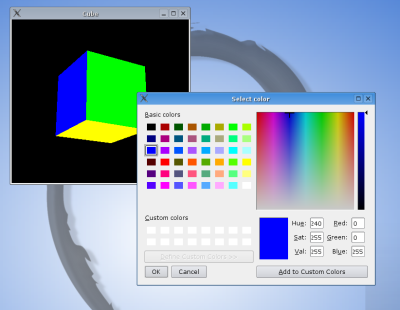
\includegraphics[width=.95\textwidth  %, clip, trim = 50mm 74mm 100mm 36mm
  ]
  {threadedcube_screenshot.png}
 %
 %\vspace{-.2cm}
\caption{Screenshot of application with active context menu after picking the left face.
}
  \label{fig:screenshot}
\end{center}
\end{figure}

We have shown how to implement multi-threaded OpenGL with picking capabilities based on Qt's OpenGL and Thread modules.
%
To this end, we combined two existing Qt sample programs~\cite{glimpse3d,Blanchette2008}.
%
The thread-safe access to the OpenGL rendering context from different threads is realized by guarding it with a mutex which gets locked and unlocked each time a thread takes temporary ownership of the rendering context.
%
A screenshot of our sample program is given in figure~\ref{fig:screenshot}.
%


This code has been licensed under the GNU Public License (GPL) and is available from {\sf mih.voxindeserto.de/threadedcube.html}.




\bibliographystyle{abbrv}


\begin{thebibliography}{10}


\bibitem{nehe32}
[1] Molofee, J., 1997-2012. {\itshape Picking, Alpha Blending, Alpha Testing, Sorting}. OpenGL Tutorial, Lesson {\bf 32}. Neon Helium Productions. http://nehe.gamedev.net/


\bibitem{glimpse3d}
[2]~Kjern\r{a}sen, T., 2003. {\itshape Glimpsing the third dimension}. Qt Quarterly {\bf 6}. Trolltech.

\bibitem%[\protect\citeauthoryear{Blanchette and Summerfield}{2008}]
{Blanchette2008}
[3]~Blanchette, J. and Summerfield, M., 2008. {\itshape C++ GUI Programming with Qt
  4}.   Prentice Hall PTR.
\end{thebibliography}

\end{document}
